\section{Sejarah \textit{Selenium}}
Kisah ini dimulai pada 2004 di ThoughtWorks di Chicago, dengan Jason Huggins membangun mode Inti sebagai JavaScriptTestRunner untuk pengujian aplikasi waktu dan Pengeluaran internal (Python, Plone). Pengujian otomatis terhadap aplikasi apa pun adalah inti dari gaya ThoughtWork, mengingat kecenderungan Agile dari konsultasi ini. Dia mendapat bantuan dari Paul Gross dan Jie Tina Wang. Bagi mereka, ini adalah pekerjaan harian.

Jason mulai memperagakan alat uji ke berbagai rekan. Banyak yang senang dengan umpan balik visual yang langsung dan intuitif, serta potensinya untuk tumbuh sebagai kerangka pengujian yang dapat digunakan kembali untuk aplikasi web lainnya.

Segera setelah tahun 2004 sesama ThoughtWorker Paul Hammant melihat demo, dan memulai diskusi tentang sumber terbuka Selenium, serta mendefinisikan mode 'didorong' Selenium di mana Anda bisa menggunakan Selenium melalui kabel dari bahasa pilihan Anda. , yang akan menyiasati 'kebijakan asal yang sama'. Rekan-rekan (saat itu) lainnya, Aslak Hellesoy dan Mike Melia, bereksperimen dengan berbagai ide untuk karya 'server', termasuk penulisan ulang halaman untuk mendapatkan kebijakan asal yang sama. Paul menulis karya server asli di Jawa, dan Aslak dan Obie Fernandez mengangkut driver klien ke Ruby, menetapkan fondasi untuk driver dalam lebih banyak bahasa.

Pekerja Pikir di berbagai kantor di seluruh dunia mengambil Selenium untuk proyek komersial, dan berkontribusi kembali ke Selenium dari pelajaran yang dipetik dari proyek ini. Mike Williams, Darrell Deboer, dan Darren Cotterill semuanya membantu meningkatkan kemampuan dan ketahanannya.

\section{Jenis-Jenis \textit{Selenium}}
Selenium adalah perangkat lunak yang berfungsi untuk mendukung pengembangan otomatisasi uji berbasis web aplikasi. Selenium menyediakan pengujian khusus terhadap domain bahasa,untuk melakukan tes menulis pada beberapa bahasa pemrograman yan populer, termasuk C, Groovy, Java, Pearl, PHP, Python, Ruby, dan juga Scala. Pengujian dapat berjalan melalui browser web apa saja dan dapat dilakukan melalui Sistem Operasi di Windows, Linux, dan Platform OS X. Selenium Python Bindings menyediakan API yang sederhana untuk menulis uji fungsional menggunakan Selenium WebDriver, dan juga dapat mengakses semua fungsi Selenium WebDriver secara intuitif. Selenium Python Bindings menyediakan API yang cukup nyaman untu melakukan suatu akses Selenium WebDrivers seperti di Firefox, Internet Explorer, Chrome, dll 

Jenis-Jenis Selenium Sebagai Berikut :

\begin{enumerate}

\item \textit{IDE selenium}
\par Selenium IDE (Lingkungan Pengembangan Terpadu) adalah sumber terbuka alat rekam dan putar untuk menghasilkan skrip Selenium, yang terintegrasi dengan browser web Firefox sebagai ekstensi. Ini adalah tes UI berbasis web yang terkenal alat otomatisasi yang mengekstrak segala jenis locator dari halaman web. Ator banyak yang bisa baik berbasis atribut atau berbasis struktur, dan termasuk ID, nama, tautan, XPath, CSS, dan DOM. IDE memiliki seluruh Selenium Core, yang memungkinkan pengguna mencatat 10, memutar, mengedit, dan men-debug tes secara manual di browser. Tindakan pengguna di web halaman dapat direkam dan diekspor dalam bahasa apa saja yang paling populer, seperti Java, C , Ruby, dan Python, Selenium Builder adalah alat open source alternatif untuk dicatat oleh Selenium IDE dan pemutaran aplikasi web. Ini adalah ekstensi dari web browwr Firefox, Yang mirip dengan Selenium IDE, tetapi, ia memiliki beberapa fitur unik yaitu Selenium IDE tidak mendukung. S'lenium Builder adalah alat standar dari Sauce Lahs yang menjalankan tes Sauce Cloud dari antarmuka Selenium Builder itu sendiri.

\item \textit{Selenium WebDriver}
\par Selenium webdriver adalah versi terbaru dari selenium IDE dan selenium Remote Control (RC). Ini juga dinamai selenium 2.0. Ini memungkinkan skrip uji yang dirancang untuk berkomunikasi dengan browser secara langsung dengan bantuan metode asli. Ini mendukung pengujian aplikasi web pada desktop serta pada perangkat seluler seperti Android dan iOS
perangkat. Biaya proyek berkurang dengan bantuan ini alat karena itu adalah alat open-source. Waktu yang diperlukan untuk mengeksekusi skrip pengujian di webdriver kurang jika dibandingkan ke selenium IDE dan Selenium RC.Ini memungkinkan skrip pengujian dirancang untuk berbagai browser seperti Internet explorer, Firefox, Mac safari dan Chrome. Script pengujian dapat dikembangkan menggunakan bahasa seperti Java, C , Ruby, Perl, Python.


\item \textit{Remote Control Selenium}
\par Remote Control Selenium (RC) adalah selenium utama yang digunakan untuk memproyeksikan waktu yang lama. Selenium RC lebih lambat daripada selenium webdriver karena menggunakan program java script yang disebut sebagai suatu inti dari selenium. Selenium RC harus memulai server sebelum menjalankan suatu skrip pengujian, dan itu tidak mendukung untuk aplikasi Ajax. Cara menghindari keterbatasan Selenium RC, aitu dengan selenium Web Driver.

\item \textit{Selenium Grid}
\par Server yang memungkinkan pengujian untuk menggunakan instace browser web yang sedang berjalan di mesin jarak jauh. Dengan selenium grid, satu server bertindak sebagai hub. Tes hubungi hub untuk mendapatkan akses ke instance browser karena hub memiliki daftar server yang menyediakan akses ke insntance browser (node WebDriver), dan memungkinkan pengujian menggunakan instance ini. Selenium Grid memiliki kemampuan untuk menjalankan tes pada instance browser jarak jauh yang berguna untuk menyebarkan beban pengujian di beberapa mesin, dan untuk menjalankan tes di browser yang berjalan pada platform atau sistem operasi yang berbeda. Yang terakhir ini sangat berguna dalam kasus di mana tidak semua browser yang akan digunakan untuk pengujian dapat berjalan pada platform yang sama.

\item \textit{TestNG} 
\par TestNG adalah kerangka pengujian yang digunakan untuk pengujian otomatisasi bersama dengan selenium 2.0.Ini mendukung berbagai tingkat pengujian seperti unit, integrasi, sistem dan pengujian penerimaan pengguna (UAT). Biasanya disebut sebagai "Uji Generasi Baru".
\end{enumerate}

\section{Geckodriver dan Chromedriver}
\subsection{Gechodriver untuk Mozilla Firefox}
\par Download Geckodriver pada link ini https://github.com/mozilla/geckodriver/releases. sebelum mendownload harus menyamakan versi mozilla dengan versi Geckodriver misal versi Mozilla firefox versi 32bit Geckodrivernya pun harus 32bit jika tidak maka akan terjadi kesalahan.

jika sudah mendownload Geckodriver pindahkan file tersebut ke system32
\begin{figure}[H]
    \centering
    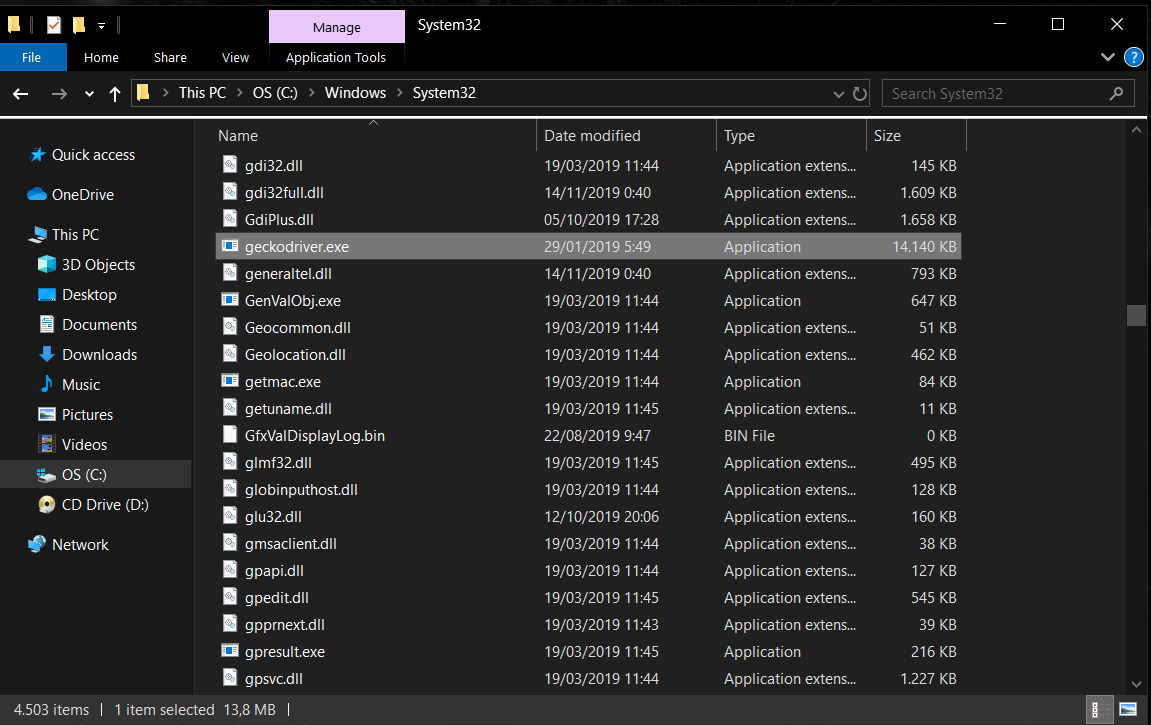
\includegraphics[scale=0.3]{Figures/figures/gechodriver}
    \caption{\textit{Gechodriver}}
    \label{Geckodriver}
\end{figure}

\section{Penggunaan Selenium}
\par Disini kami mencoba menjalankan otomasi \textit{web testing} menggunakan \textit{python} dan dengan menggunakan \textit{IDE Spyder}.
Langkah-langkahnya yaitu :
\begin{enumerate}
\item buka \textit{spyder} dan tampilan awalnya seperti ini :
	\begin{figure}[H]
    	\centering
    	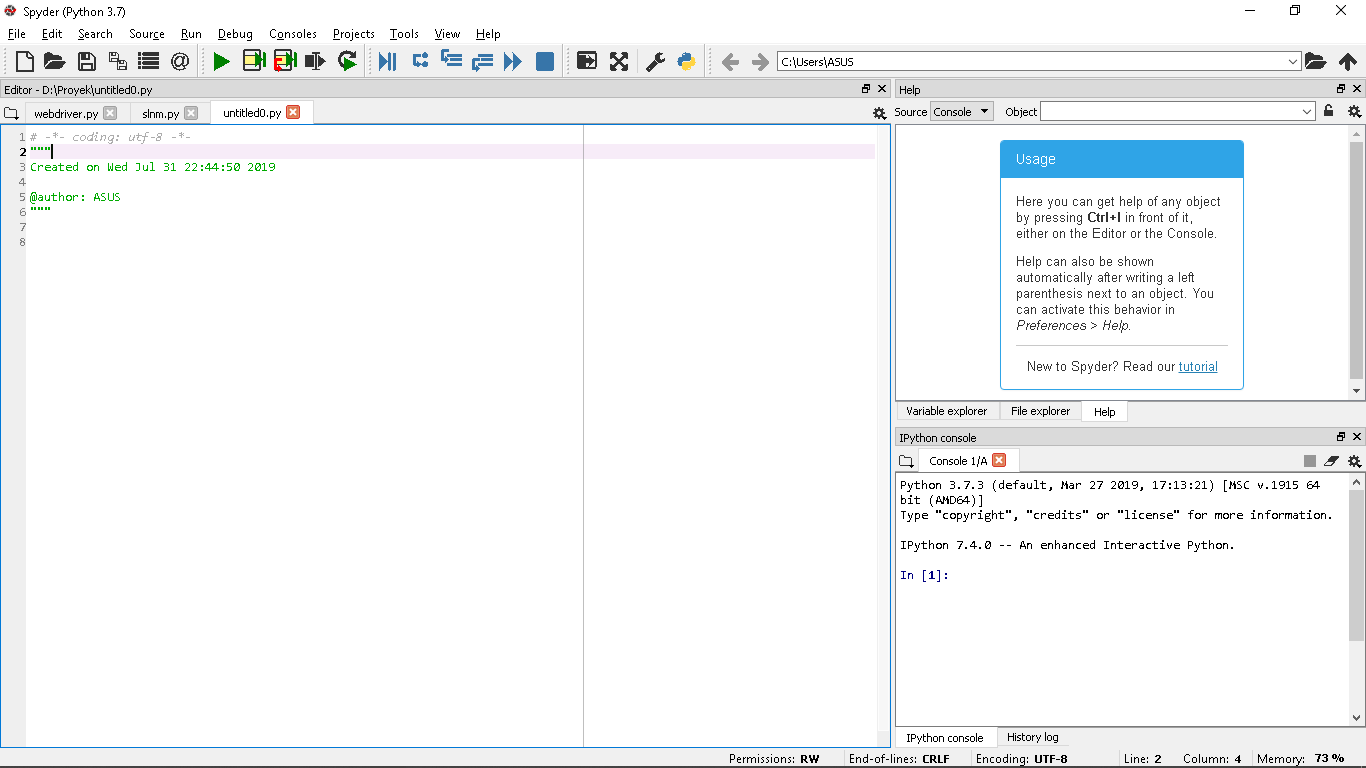
\includegraphics[scale=0.3]{Figures/figures/awalspy.png}
    	\caption{\textit{Tampilan awal spyder}}
    	\label{CLI}
	\end{figure}
	
\item kemudian ketikkan codingan:
\begin{lstlisting}[language=Python]
from selenium.webdriver import Firefox
from selenium.webdriver.firefox.options import Options
from selenium.webdriver.common.desired_capabilities import DesiredCapabilities
from selenium.webdriver.firefox.firefox_binary import FirefoxBinary

print("Masukkan Npm Anda:")
npm = input()
print("Masukkan Password SIAP Anda:")
paswd = input('')

opsi = Options()

opsi.headless = False
binary = FirefoxBinary("C:\\Program Files\\Mozilla Firefox\\firefox.exe")
cap = DesiredCapabilities().FIREFOX
cap['marionette'] = True

browser=Firefox(executable_path='geckodriver.exe',
options=opsi,capabilities=cap,firefox_binary=binary)
browser.get('http://siap.poltekpos.ac.id/siap/besan.depan.php')

name = browser.find_element_by_name('user_name')
word = browser.find_element_by_name('user_pass')
login = browser.find_element_by_name('login')


name.send_keys(npm)
word.send_keys(paswd)
login.click()

\end{lstlisting}

Penjelasan Codingan :
\begin{lstlisting}[language=Python]
from selenium.webdriver import Firefox
\end{lstlisting}
Yaitu Modul selenium webdriver mengimplementasikan kelas yang mendukung berbagai browser termasuk Firefox, Chrome, Internet Explorer, Safari, yang lain, dan RemoteWebDri	ver juga untuk menguji pada browser yang tersedia di mesin jarak jauh. Kita perlu mengimpor webdriver dari paket Selenium untuk menggunakan metode Selenium WebDriver.

\begin{lstlisting}[language=Python]
from selenium.webdriver.firefox.options import Options
\end{lstlisting}
Yaitu Opsi kelas dalam paket webdriver selenium firefox. opts adalah turunan dari kelas Opsi yang dipakai untuk program.

\begin{lstlisting}[language=Python]
from selenium.webdriver.common.desired_capabilities import DesiredCapabilities
\end{lstlisting}
Webdriver.common.desired\_capabilities import DesiredCapabilities()
sebagai titik awal untuk membuat objek kemampuan yang diinginkan untuk meminta driver web jarak jauh untuk terhubung ke server selenium.

\begin{lstlisting}[language=Python]
from selenium.webdriver.firefox.firefox_binary import FirefoxBinary
\end{lstlisting}
Yaitu untuk mengimport FirefoxBinary atau lokasi dari si firefox.

\begin{lstlisting}[language=Python]
print("Masukkan Npm Anda:")
npm = input()
print("Masukkan Password SIAP Anda:")
paswd = input('')

\end{lstlisting}
ini merupakan inputan \textit{user}

\begin{lstlisting}[language=Python]
browser.get('http://siap.poltekpos.ac.id/siap/besan.depan.php')
\end{lstlisting}
Browser.get metode akan menavigasi ke halaman yang diberikan oleh URL. WebDriver akan menunggu hingga halaman dimuat penuh (yaitu, "download" telah diaktifkan) sebelum mengembalikan kontrol ke tes atau skrip.

\item Setelah membuat Tambahan Codingan  seperti diatas untuk merunning program anda tekan run pada bar diatas.
\begin{figure}[H]
    	\centering
    	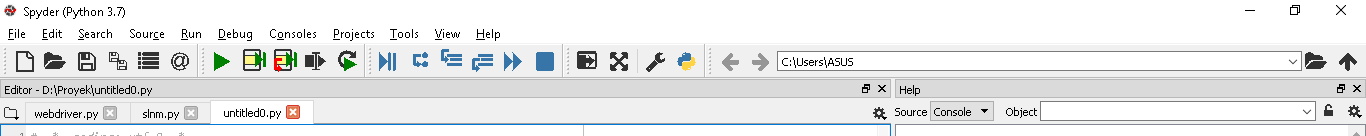
\includegraphics[scale=0.3]{Figures/figures/run1.png}
    	\caption{\textit{Running spyder}}
    	\label{CLI}
	\end{figure}

\newpage

\item Pada saat di run akan terlihat pada IPython console seperti gambar 
\begin{figure}[H]
    	\centering
    	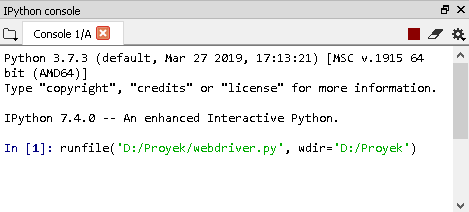
\includegraphics[scale=0.5]{Figures/figures/run2.png}
    	\caption{\textit{Running spyder console}}
    	\label{CLI}
	\end{figure}

\item Saat kotak yang ditandai pada gambar dibawah, berwarna merah artinya proses running program tersebut masih berjalan.
\begin{figure}[H]
    	\centering
    	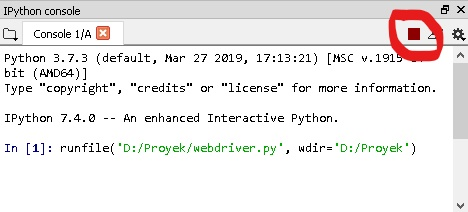
\includegraphics[scale=0.5]{Figures/figures/run3.png}
    	\caption{\textit{Running masih berjalan}}
    	\label{CLI}
	\end{figure}

\item Jika proses \textit{running} sudah selesai tampilannya akan seperti ini. Berarti Tambahan Codingan tersebut berhasil di \textit{running} dan tidak terdapat \textit{error}.
\begin{figure}[H]
    	\centering
    	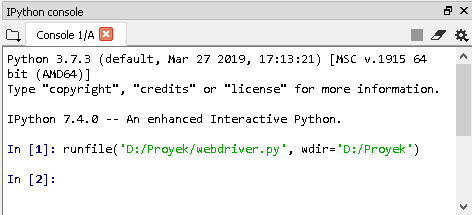
\includegraphics[scale=0.5]{Figures/figures/run4.png}
    	\caption{\textit{Running selesai}}
    	\label{CLI}
	\end{figure}

\item Setelah program di run akan otomatis membuka Mozila Firefox dan akan langsung membuka website siap.poltekpos.ac.id secara otomatis.
\begin{figure}[H]
    	\centering
    	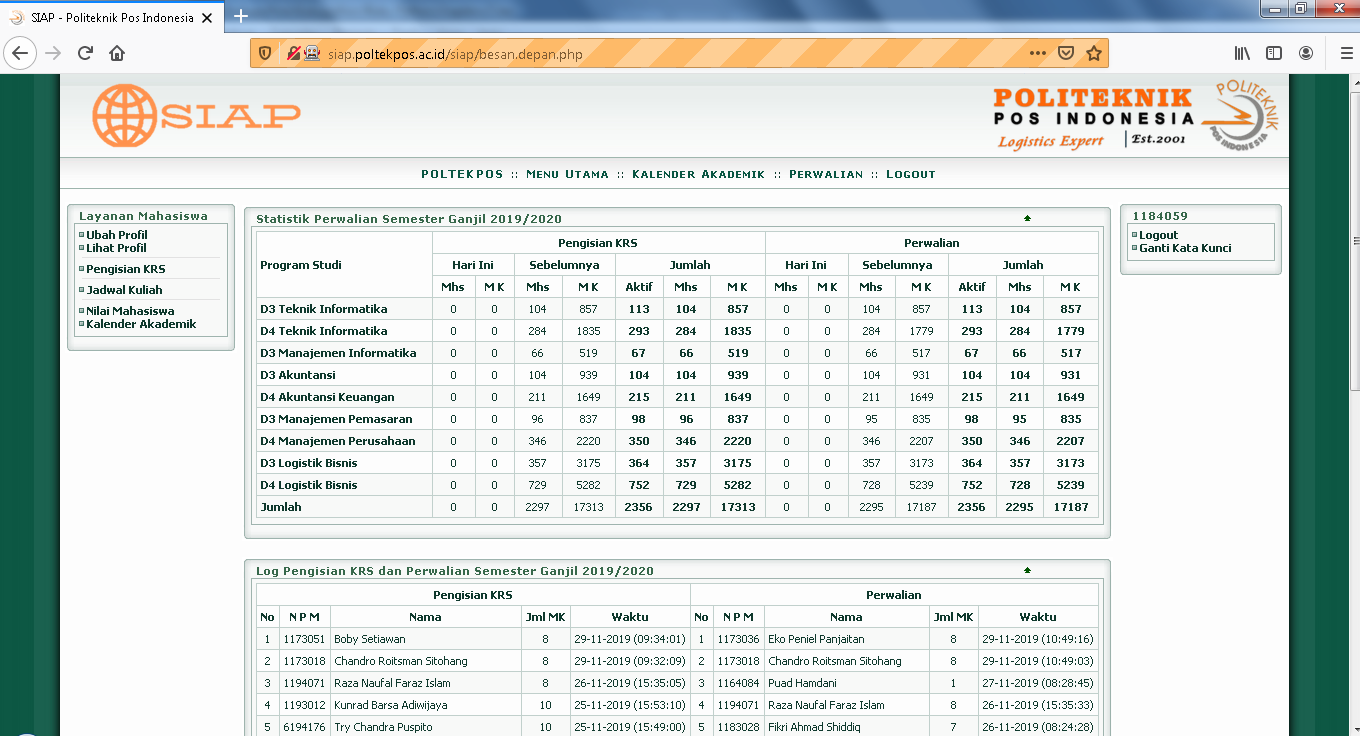
\includegraphics[scale=0.3]{Figures/figures/run5.png}
    	\caption{\textit{Tampilan siap.poltekpos}}
    	\label{CLI}
	\end{figure}


\end{enumerate}

\subsection{Cara find element atau class }
\par Selanjutnya kami akan mencoba \textit{Find Element} yang terdapat pada \textit{website} tersebut. Sebelumnya anda harus mengetahui apa saja jenis-jenis \textit{element} dan berikut adalah contoh dari \textit{element}.

\begin{enumerate}
\item find\_element\_by\_id
\par Gunakan ini ketika Anda tahu atribut id suatu elemen. Dengan strategi ini, elemen pertama dengan nilai atribut id yang cocok dengan lokasi akan dikembalikan.
contoh :
\begin{lstlisting}[language=Python]
<form id="login">
   login = Browser.find_element_by_id('login')
\end{lstlisting}

\item find\_element\_by\_name
\par Gunakan ini ketika Anda tahu atribut nama elemen. Dengan strategi ini, elemen pertama dengan nilai atribut nama yang cocok dengan lokasi akan dikembalikan.
contoh :
\begin{lstlisting}[language=Python]
<input name ="username" type="text" />
  username = Browser.find_element_by_name('username')
\end{lstlisting}

\item find\_element\_by\_xpath
\par XPath adalah bahasa yang digunakan untuk menemukan node dalam dokumen XML. Karena HTML dapat menjadi implementasi XML (XHTML), pengguna Selenium dapat memanfaatkan bahasa yang kuat ini untuk menargetkan elemen dalam aplikasi web mereka. Dan cara mendapatkan xpath adalah inspect website tersebut dan klik kanan pada element yang ingin di cari dan klik copy dan disana ada copy Xpath.
contoh :
\begin{lstlisting}[language=Python]
" ('/html/body/table/tbody/tr[5]/td/table[3]/tbody/tr[1]/td[2]/p[1]/table/tbody/tr/td[3]/select').click()" 
 browser.find_element_by_xpath('/html/body/table/tbody/tr[5]/td/table[3]/tbody/tr[1]/td[2]/p[1]/table/tbody/tr/td[3]/select').click()
\end{lstlisting}

\item find\_element\_by\_link\_text
\par Gunakan ini ketika Anda tahu teks tautan yang digunakan dalam tag jangkar. Dengan strategi ini, elemen pertama dengan nilai teks tautan yang cocok dengan lokasi akan dikembalikan. 
contoh :
\begin{lstlisting}[language=Python]
<a href="continue.html">Continue</a>
Continue = Browser.find_element_by_link_text('Continue')
\end{lstlisting}

\item find\_element\_by\_tag\_name
\par Gunakan ini ketika Anda ingin mencari elemen dengan nama tag. Dengan strategi ini, elemen pertama dengan nama tag yang diberikan akan dikembalikan.
contoh :
\begin{lstlisting}[language=Python]
<strong>Hello</strong> 
Strong = Browser.find_element_by_tag_name('strong')
\end{lstlisting}

\item find\_element\_by\_class\_name
\par Gunakan ini ketika Anda ingin mencari elemen dengan nama atribut kelas. Dengan strategi ini, elemen pertama dengan nama atribut kelas yang cocok akan dikembalikan. 
contoh :
\begin{lstlisting}[language=Python]
<p class="body">Halo.</p>
body = Browser.find_element_by_class_name('body')
\end{lstlisting}

\item find\_element\_by\_css\_selector
\par Gunakan ini ketika Anda ingin mencari elemen dengan sintaks pemilih CSS. Dengan strategi ini, elemen pertama dengan pemilih CSS yang cocok akan dikembalikan. 
contoh : 
\begin{lstlisting}[language=Python]
<p class="body">Halo.</p> 
body = Browser.find_element_by_class_name('p.body')
\end{lstlisting}

\end{enumerate}

\subsection{Mengambil element dari web siap.poltekpos.ac.id}
\par Setelah mengenal tentang element mari kita mencoba mencari element pada website siap.poltekpos.ac.id
\newpage

\begin{enumerate}
\item Disini kami mencoba untuk mengisi data \textit{user} pada \textit{login}.
\begin{figure}[H]
    	\centering
    	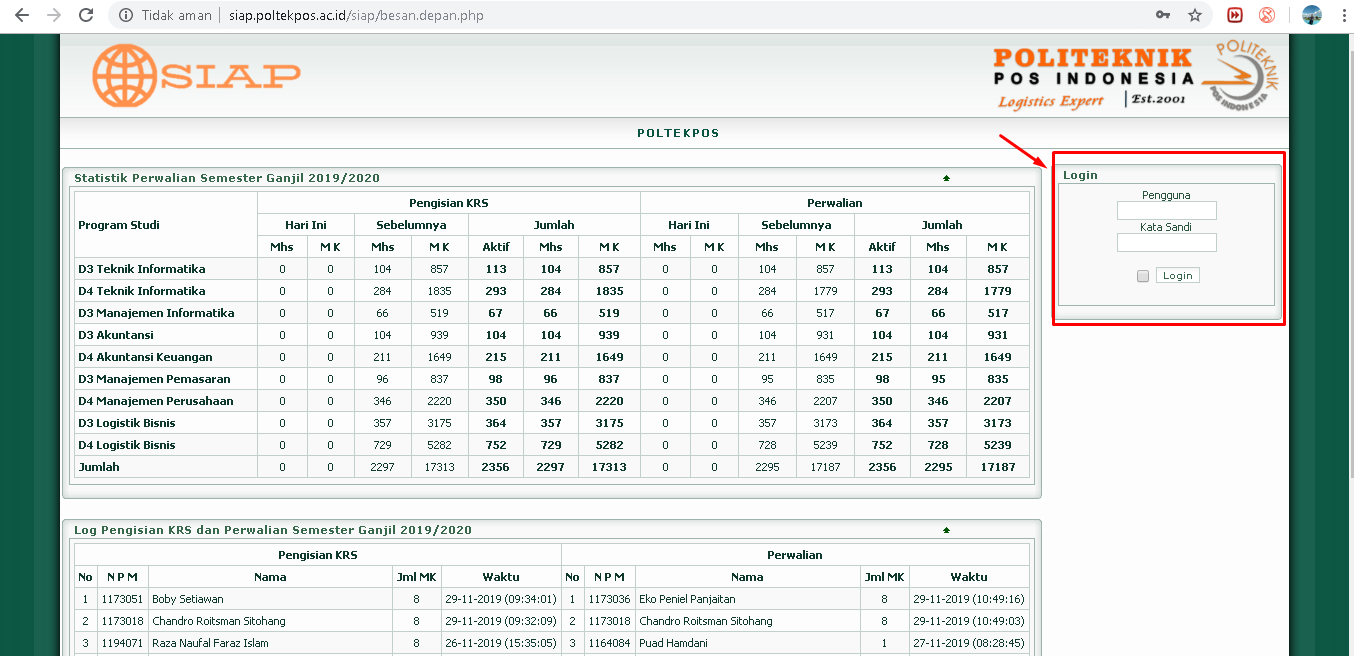
\includegraphics[scale=0.3]{Figures/figures/siap.png}
    	\caption{\textit{Tampilan siap.poltekpos}}
    	\label{CLI}
	\end{figure}
\item Untuk mencari elementnya arahkan cursor ke \textit{login} pengguna, kata sandi, dan login. lalu klik kanan dan \textit{inspect}, disini kami menggunakan element\_by\_name.

\begin{figure}[H]
    	\centering
    	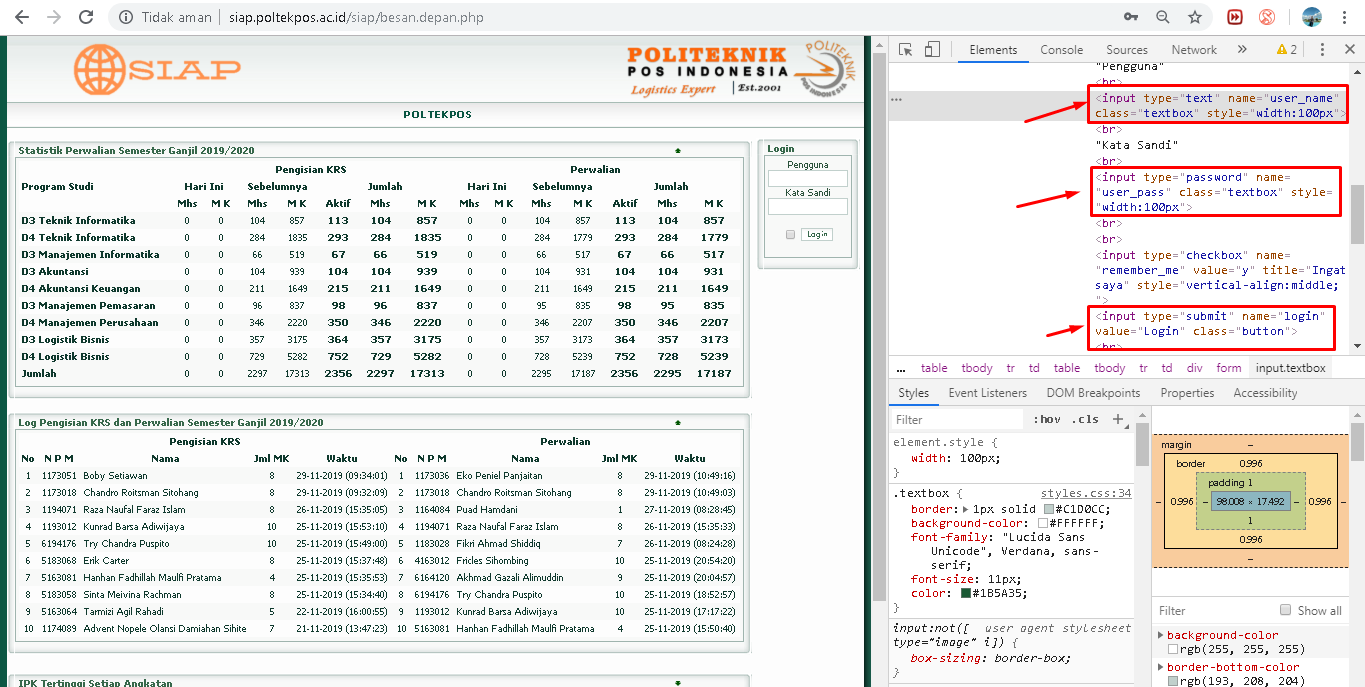
\includegraphics[scale=0.3]{Figures/figures/inspect1.png}
    	\caption{\textit{inspect element by name}}
    	\label{CLI}
	\end{figure}
	
Tambahan Codingan :
\begin{lstlisting}[language=Python]
name = browser.find_element_by_name('user_name')
word = browser.find_element_by_name('user_pass')
login = browser.find_element_by_name('login')

\end{lstlisting}

\newpage

Hasil :
\begin{figure}[H]
    	\centering
    	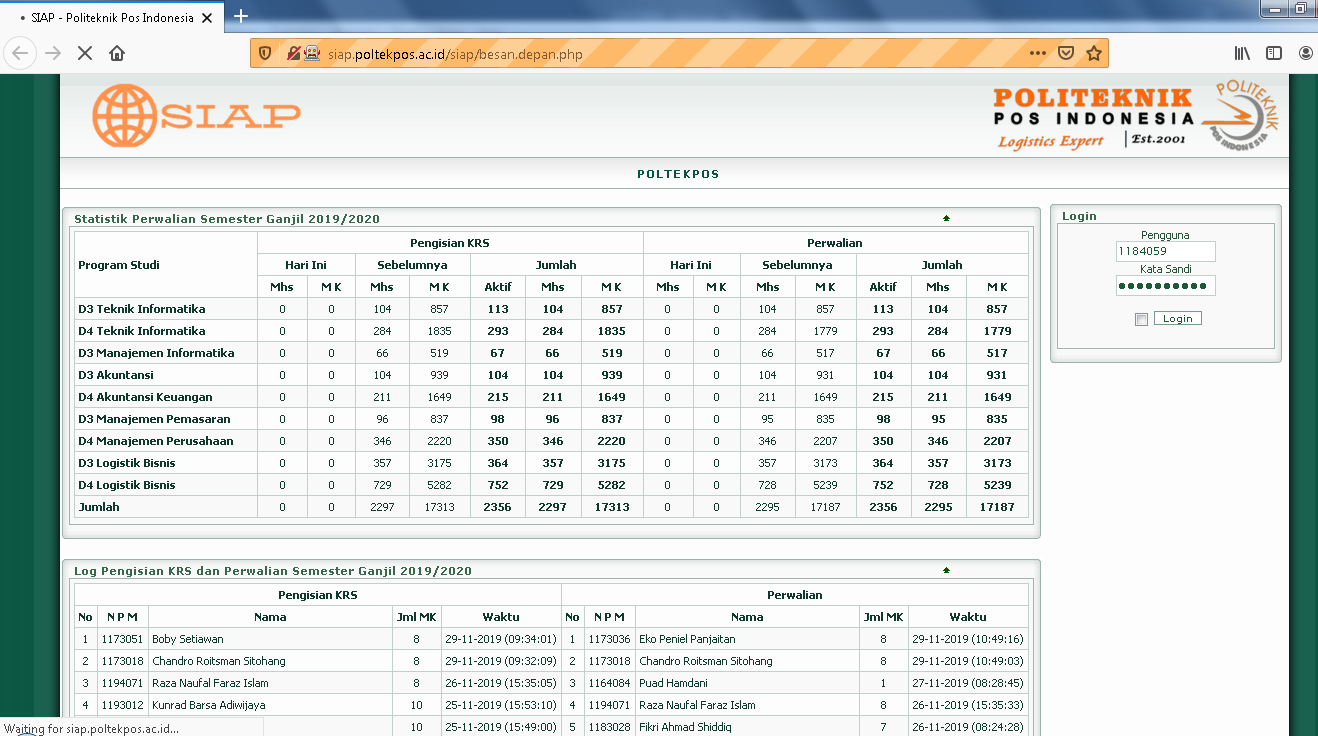
\includegraphics[scale=0.3]{Figures/figures/hasillogin.png}
    	\caption{\textit{Tampilan loading login}}
    	\label{CLI}
	\end{figure}
	
Hasil :
\begin{figure}[H]
    	\centering
    	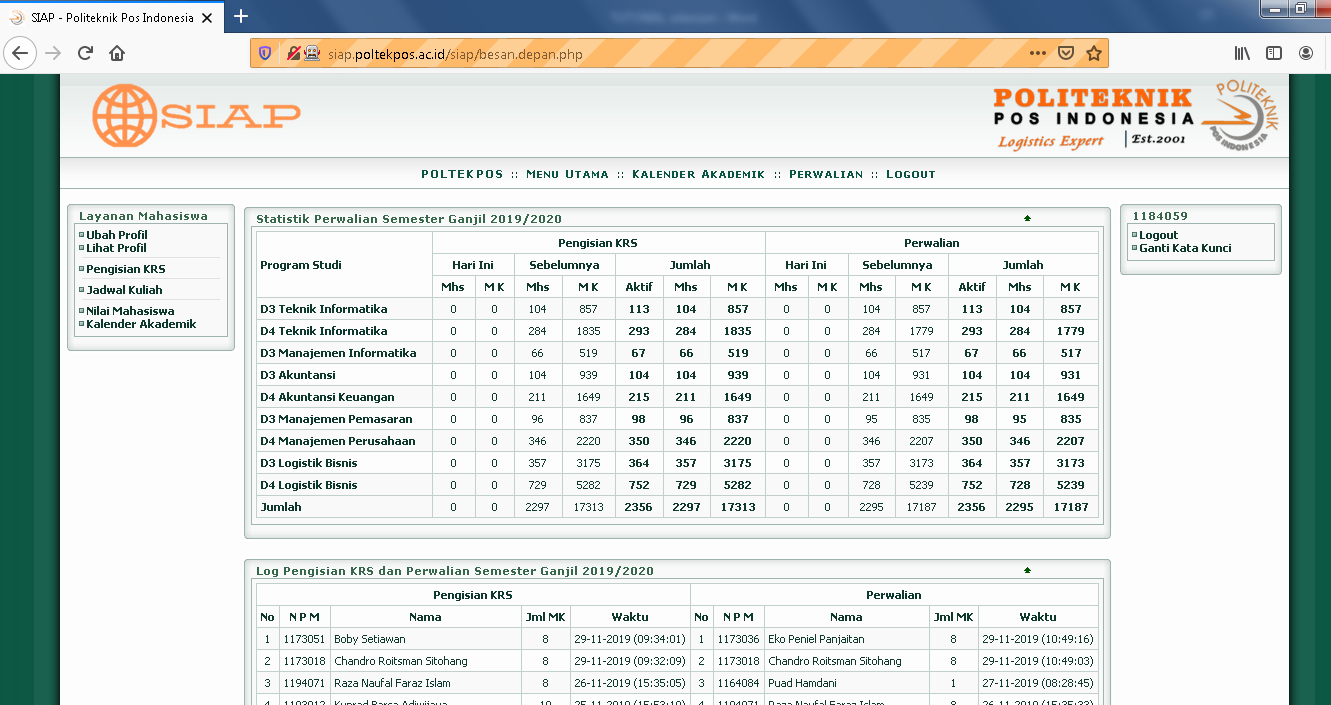
\includegraphics[scale=0.3]{Figures/figures/hasillogin1.png}
    	\caption{\textit{Tampilan login}}
    	\label{CLI}
	\end{figure}


\item Pada layanan mahasiswa, kami mencoba untuk melihat nilai mahasiswa secara otomatis. Dengan cara yaitu klik kanan pada nilai mahasiswa, kemudian pilih \textit{inspect}.
\begin{figure}[H]
    	\centering
    	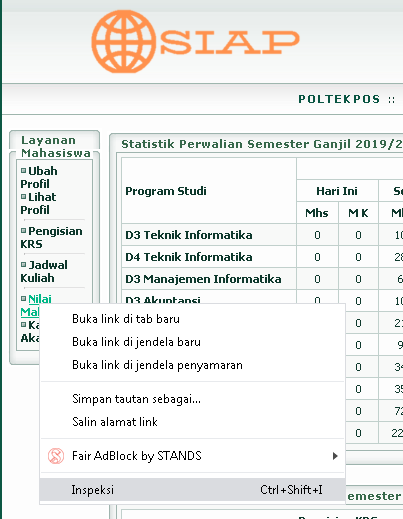
\includegraphics[scale=0.5]{Figures/figures/nilai1.png}
    	\caption{\textit{inspect element nilai mahasiswa}}
    	\label{CLI}
	\end{figure}

\newpage

Disini kami mengambil \textit{element by xpath}
\begin{figure}[H]
    	\centering
    	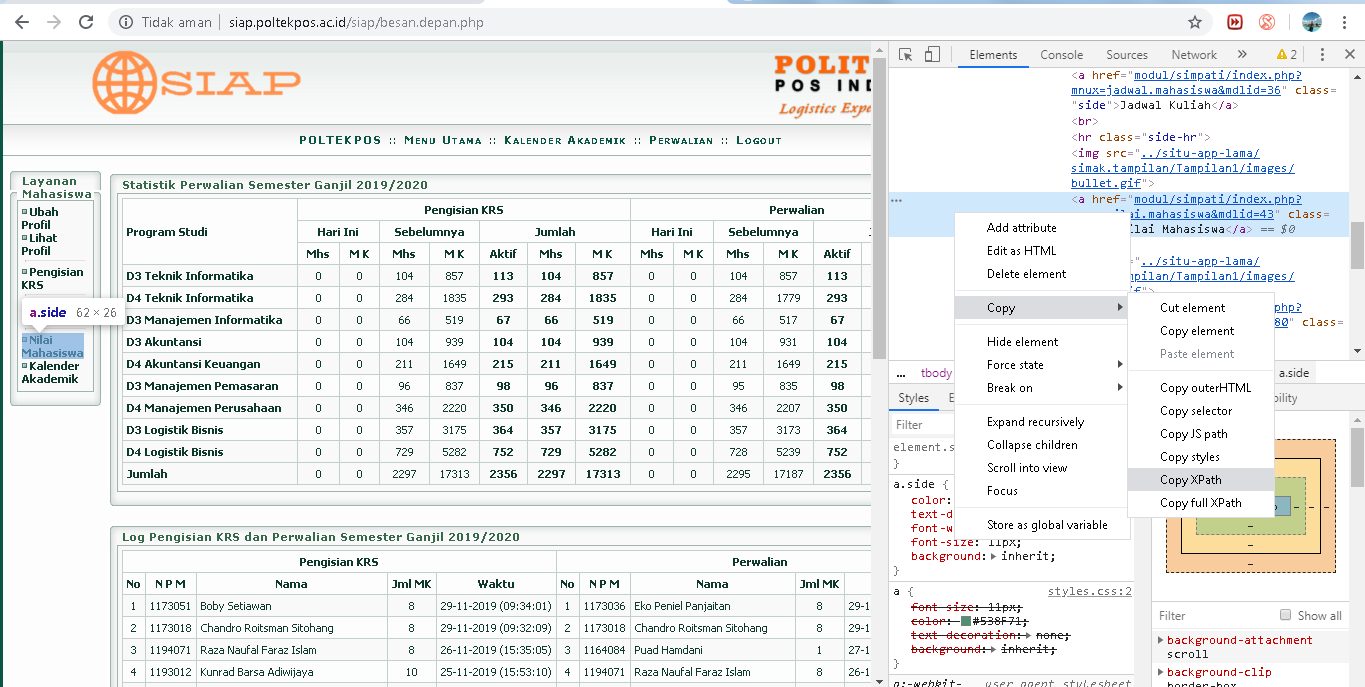
\includegraphics[scale=0.3]{Figures/figures/nilai2.png}
    	\caption{\textit{inspect element by xpath}}
    	\label{CLI}
	\end{figure}
	
Tambahan codingan :
\begin{lstlisting}[language=Python]
nilai= browser.find_element_by_xpath("/html/body/table/tbody/tr[5]/td/table[1]/tbody/tr/td[1]/table[2]/tbody/tr[1]/td[2]/a[5]").click()
\end{lstlisting}

Hasil :
\begin{figure}[H]
    	\centering
    	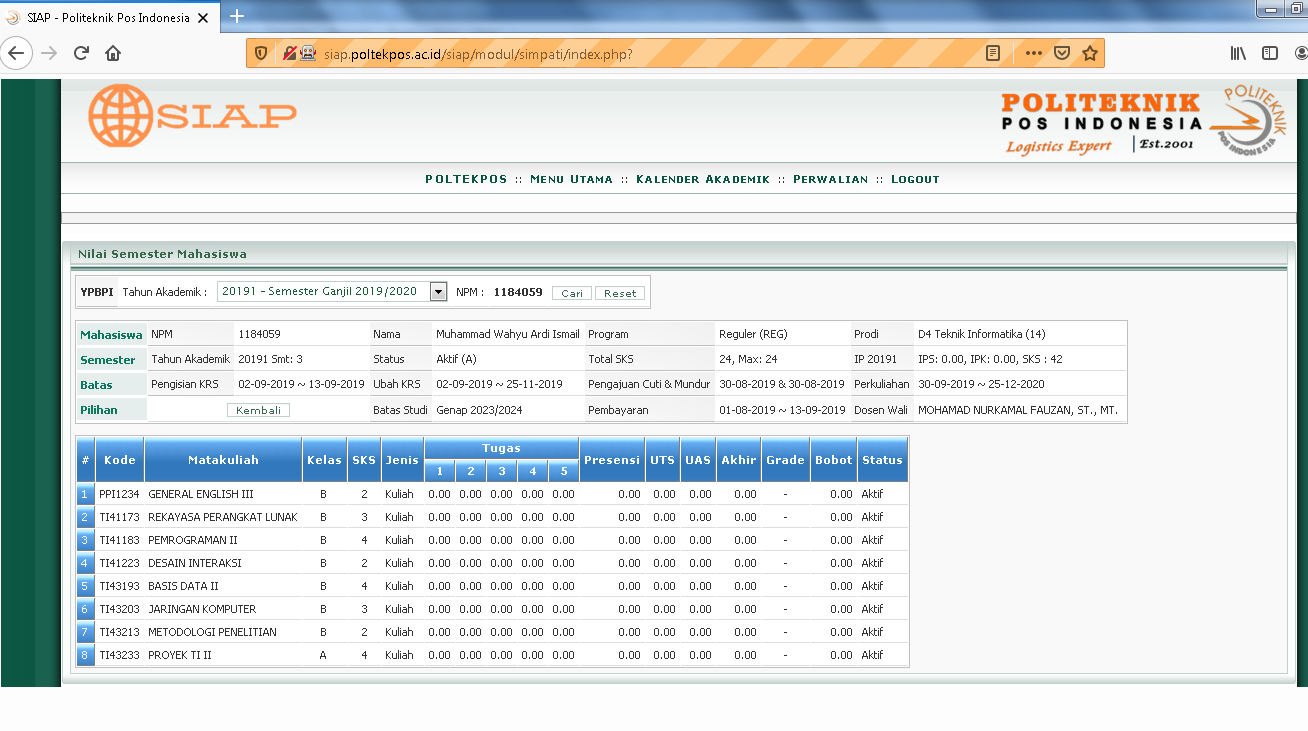
\includegraphics[scale=0.3]{Figures/figures/hasilnilai1.png}
    	\caption{\textit{Tampilan nilai semester mahasiswa}}
    	\label{CLI}
	\end{figure}

\newpage
	
\item Kemudian pada kolom tahun akademik, klik kanan dan pilih \textit{inspect}
\begin{figure}[H]
    	\centering
    	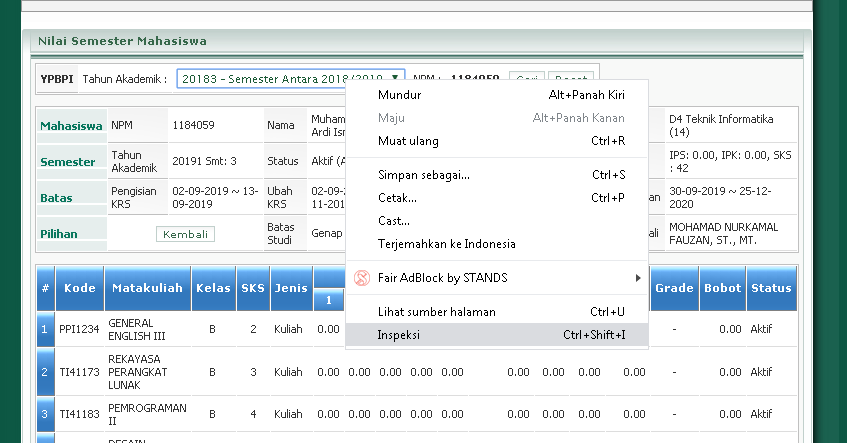
\includegraphics[scale=0.3]{Figures/figures/tahun1.png}
    	\caption{\textit{inspect element tahun akademik}}
    	\label{CLI}
	\end{figure}
	
Disini kami mengambil \textit{element by xpath} pada semester genap 2018/2019
\begin{figure}[H]
    	\centering
    	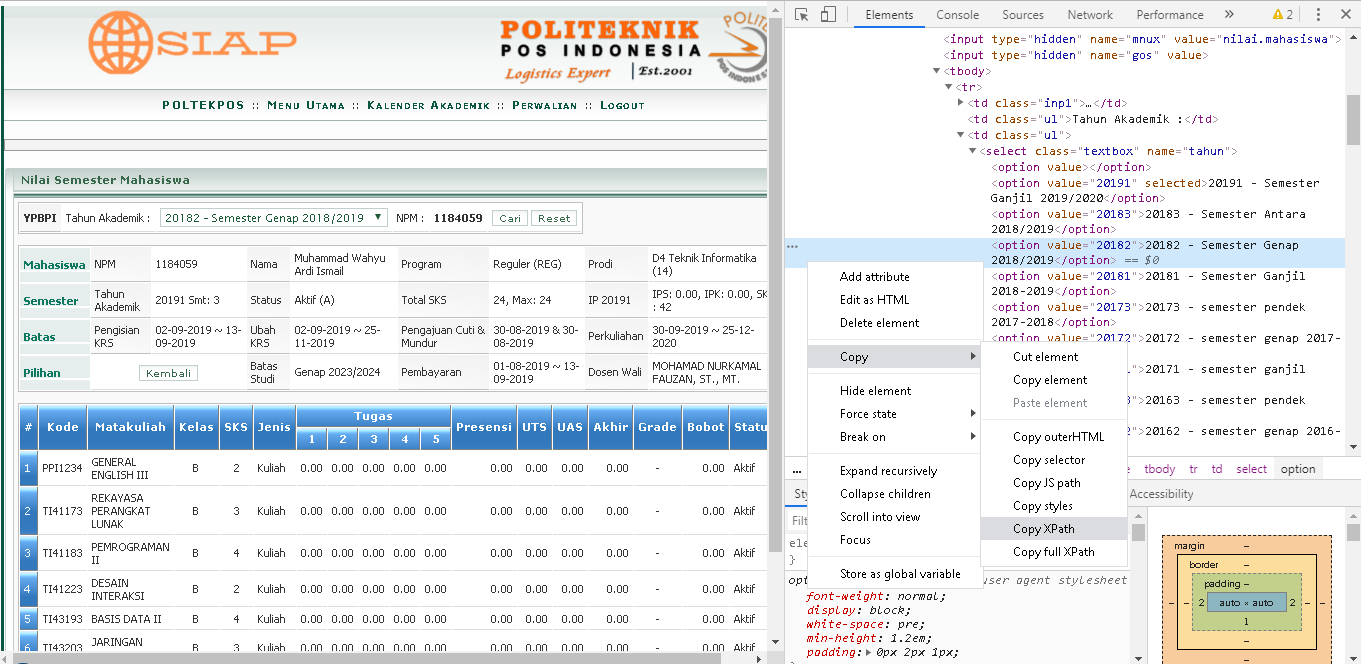
\includegraphics[scale=0.3]{Figures/figures/semestergenap.png}
    	\caption{\textit{inspect element by xpath semster genap}}
    	\label{CLI}
	\end{figure}

Tambahan codingan :
\begin{lstlisting}[language=Python]
nilai semester genap =browser.find_element_by_xpath('/html/body/table/tbody/tr[5]/td/table[3]/tbody/tr[1]/td[2]/p[1]/table/tbody/tr/td[3]/select/option[4]').click()
\end{lstlisting}

\newpage

Hasil :
\begin{figure}[H]
    	\centering
    	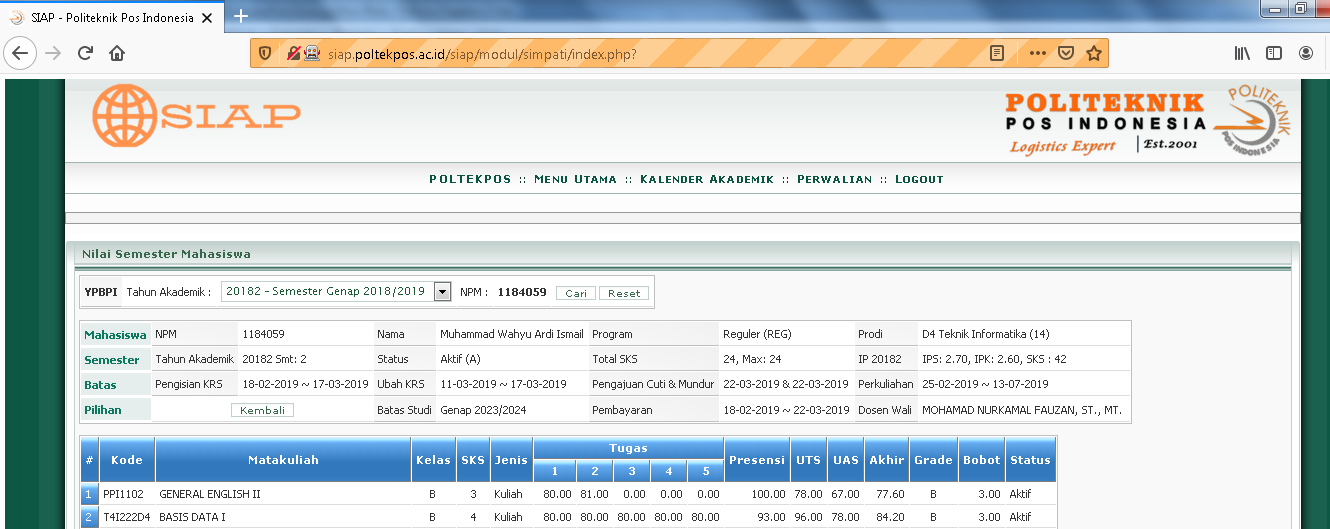
\includegraphics[scale=0.3]{Figures/figures/hasilnilai2.png}
    	\caption{\textit{Tampilan nilai semester genap 2018/2019}}
    	\label{CLI}
	\end{figure}



\item kemudian klik find cari dengan cara klik kanan pilih \textit{inspect}
\begin{figure}[H]
    	\centering
    	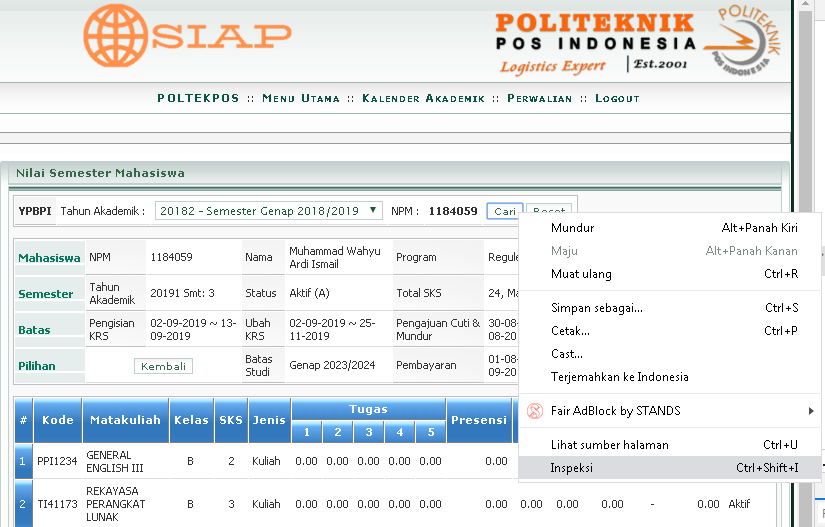
\includegraphics[scale=0.3]{Figures/figures/cari1.png}
    	\caption{\textit{inspect element cari}}
    	\label{CLI}
	\end{figure}
	
Disini kami mengambil \textit{element by class name}, \textit{class name} yaitu \textit{button}.
\begin{figure}[H]
    	\centering
    	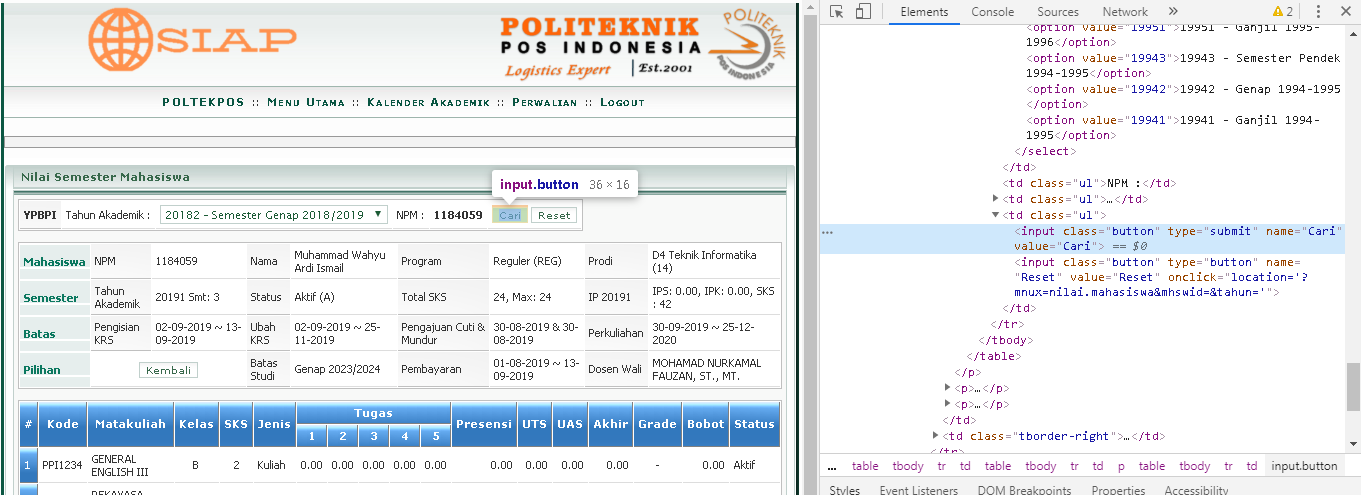
\includegraphics[scale=0.3]{Figures/figures/button1.png}
    	\caption{\textit{inspect element by class name cari}}
    	\label{CLI}
	\end{figure}

Tambahan codingan :
\begin{lstlisting}[language=Python]
cari = browser.find_element_by_class_name('button').click()
\end{lstlisting}


\item codingan keseluruhan :
\begin{lstlisting}[language=Python]
from selenium.webdriver import Firefox
from selenium.webdriver.firefox.options import Options
from selenium.webdriver.common.desired_capabilities import DesiredCapabilities
from selenium.webdriver.firefox.firefox_binary import FirefoxBinary

print("Masukkan Npm Anda:")
npm = input()
print("Masukkan Password SIAP Anda:")
paswd = input('')

opsi = Options()

opsi.headless = False
binary = FirefoxBinary("C:\\Program Files\\Mozilla Firefox\\firefox.exe")
cap = DesiredCapabilities().FIREFOX
cap['marionette'] = True

browser=Firefox(executable_path='geckodriver.exe',
options=opsi,capabilities=cap,firefox_binary=binary)
browser.get('http://siap.poltekpos.ac.id/siap/besan.depan.php')

name = browser.find_element_by_name('user_name')
word = browser.find_element_by_name('user_pass')
login = browser.find_element_by_name('login')


name.send_keys(npm)
word.send_keys(paswd)
login.click()

nilai = browser.find_element_by_xpath("/html/body/table/tbody/tr[5]/td/table[1]/tbody/tr/td[1]/table[2]/tbody/tr[1]/td[2]/a[5]").click()
semester1 = browser.find_element_by_xpath('/html/body/table/tbody/tr[5]/td/table[3]/tbody/tr[1]/td[2]/p[1]/table/tbody/tr/td[3]/select/option[4]').click()
cari = browser.find_element_by_class_name('button').click()

\end{lstlisting}

\end{enumerate}

\section{ WebDriver Exception : Can not connect to the service geckodriver}
Cara mengatasinya yaitu dengan menyamakan versi python, mozilla firefox, geckodriver , misalnya versi 64bit. Jika masih tidak bisa, silahkan buka localhost pada laptop atau komputer anda. Lokasi localhost berada di (C: Windows System32 drivers etc) kemudian buka file hosts dan edit menggunakan notepad++ kemungkian error karena di hosts 127.0.0.1


\section{SessionNotCreatedException : Unable to find a matching set of capabilities}
Cara mengatasinya yaitu dengan pada desktop klik kanan pada mozilla firefox, pilih properties dan copy pada bagian lokasi direktori Jika sudah paste kedalam kode program pada binnary mozilla firefox


\section{Module Notfound Error : no module named selenium}
Cara mengatasinya:
\begin{enumerate}
\item  uninstall aplikasi berbahasa pemrograman python, selain anaconda karena nanti akan terjadi konflik
\item restart komputer anda 
\item setting environtment kembali
\item buka cmd
\item install kembali selenium 
\item selesai
\end{enumerate} 

\section{ WebDriverExecption: cant load profile Possible version mismatch}
Cara mengatasinya cukup mengupdate versi Mozilla Firefox atau Chrome agar bisa compatible dengan drivernya.